\subsection{QRS algorithm: peak detection}
\label{sx:QRSalg}
Peak detection is invoked with a single function call in \texttt{main.c}. We implemented the algorithm similar to the template, with certain differences. All variables used in peak detection are stored in the struct \texttt{data}. \texttt{data} contains all used variables and arrays of length 33: filtered data, Rpeaks etc. The term "Rpeak" originates from the QRS complex\footnote{QRS complex described in "02131 Assignment 1: Software implementation of a personal ECG scanner"}, used to describe the profile of a heartbeat in a signal vs time plot. The "R" is the point for the main heartbeat with the largest amplitude, hence we use "Rpeak" for the main peak of interest.\\
\\
The algorithm is implemented in \texttt{qsr.c} in five functions, and the control flow resembles the template, see Fig \ref{fig:QRS_flowchart}. All tests (\color{blue} \texttt{if} \color{black} statements) are carried out by the function preceding the test.
% Hvordan er algoritmen implementeret og hvordan gemmes relevant data (R-peak)

\begin{figure}[H]
    \centering
    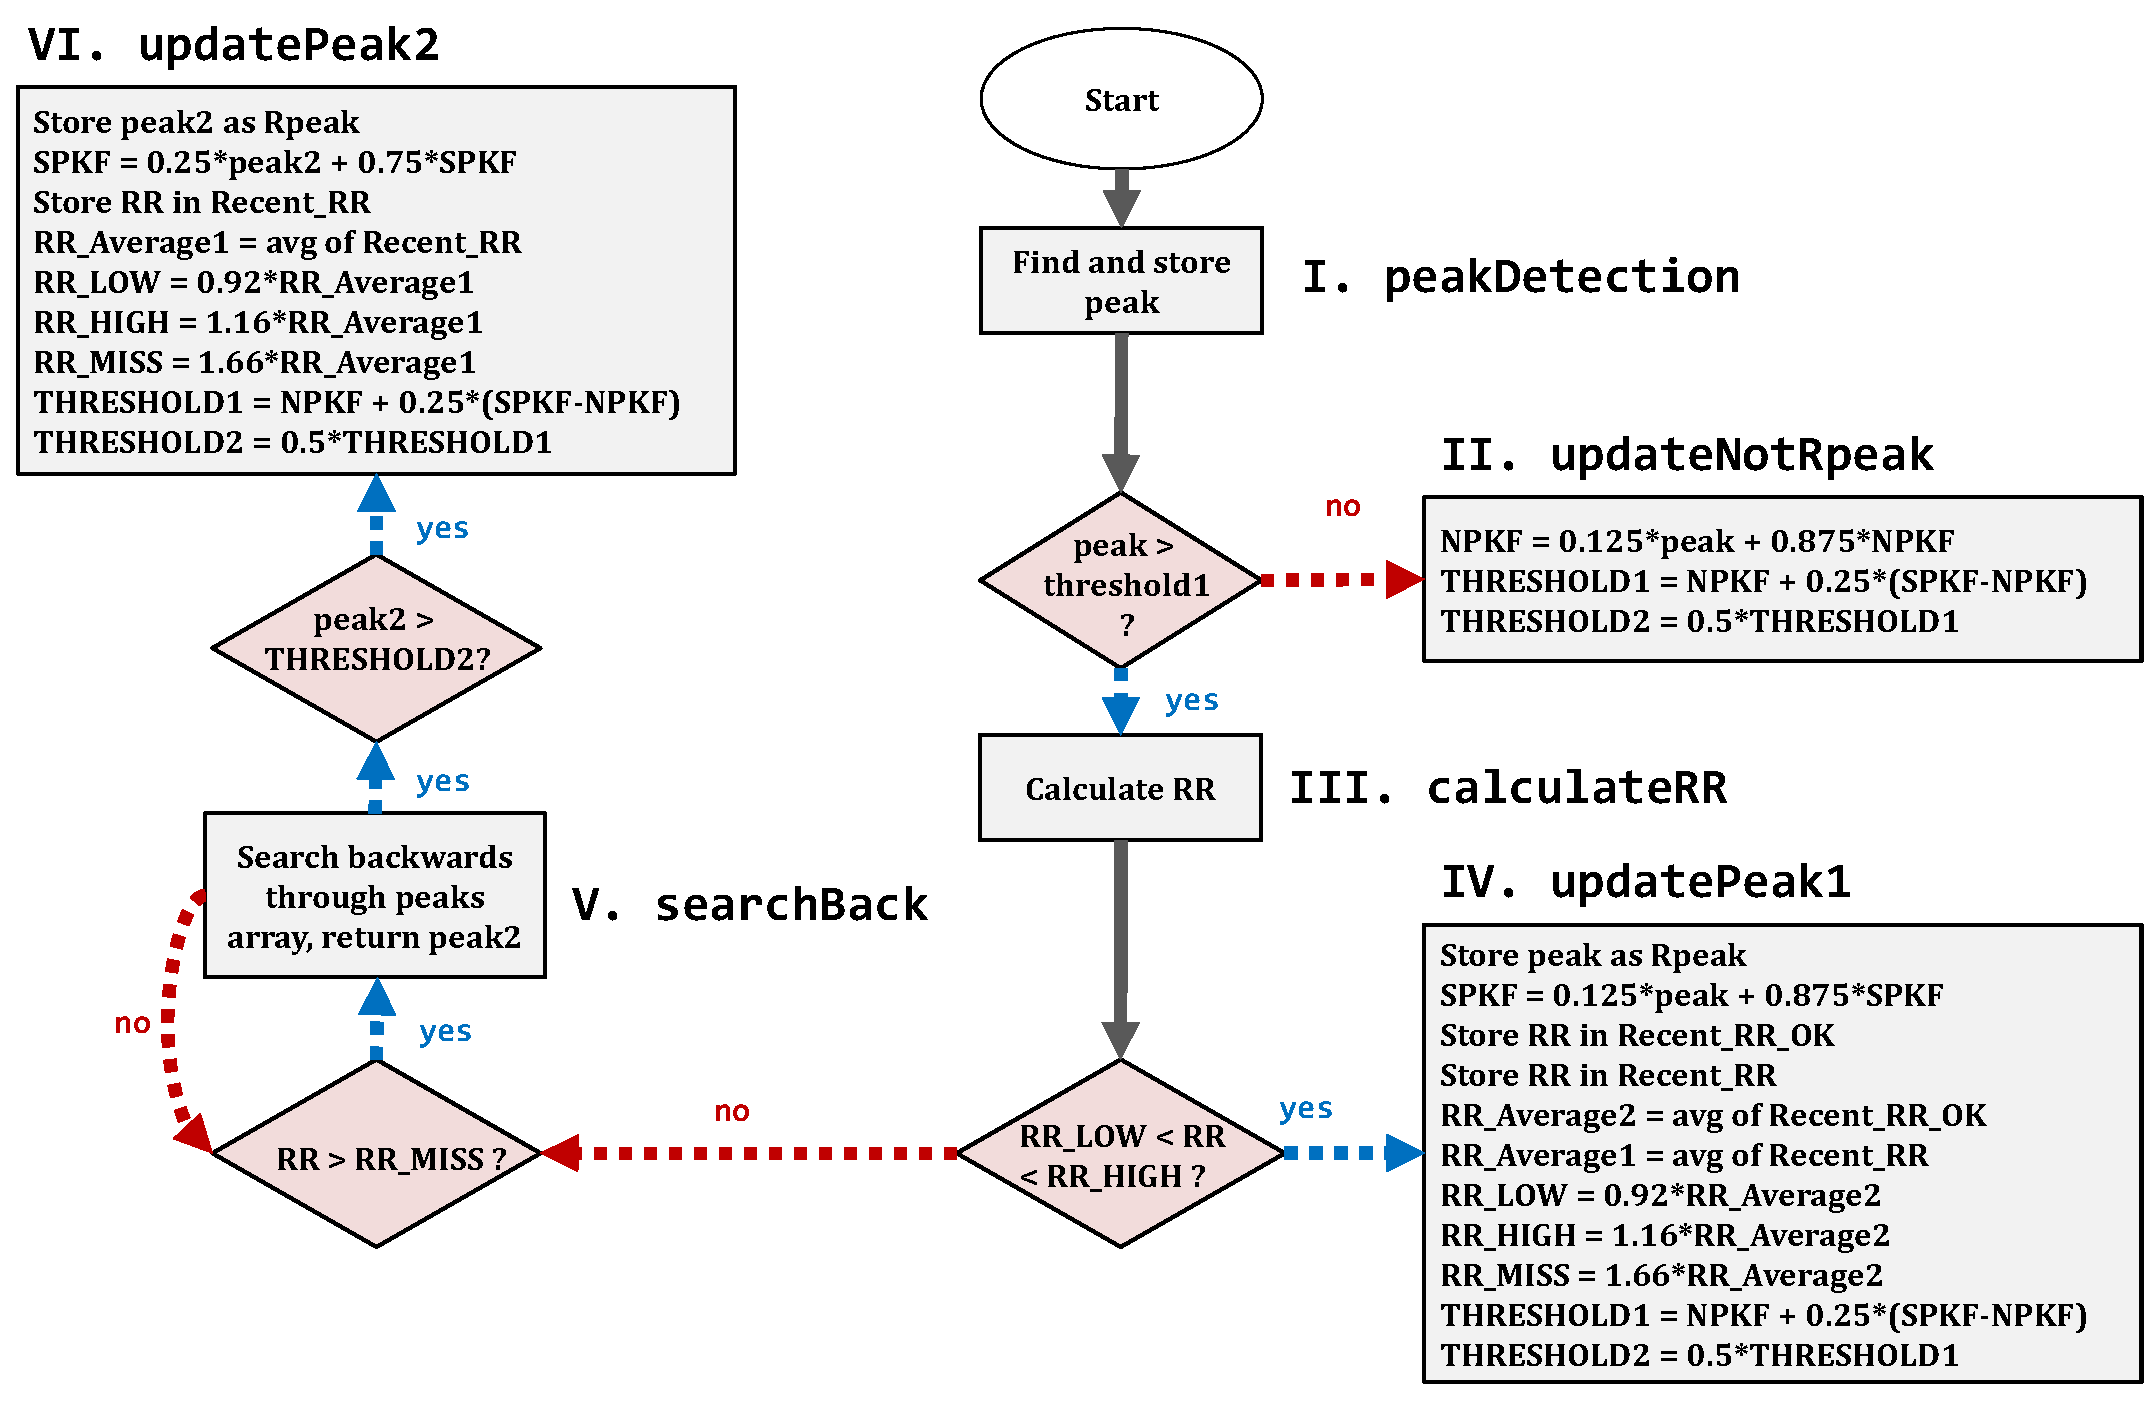
\includegraphics[width=1.0\textwidth]{1Design/fig/QRS.pdf}
    \caption{QRS algorithm flow chart, with our 6 \texttt{qrs.c} functions marked.}
    \label{fig:QRS_flowchart}
\end{figure}

In the numerated sections below, it is described how the QRS algorithm shown in figure \ref{fig:QRS_flowchart} is implemented, and how relevant data is saved for later use (e.g. R-peaks):

\subsubsection*{I. Peak detection}
In order to determine whether a peak has occurred, the last four data points ($x_n, x_{n-1}, x_{n-2}$ and $x_{n-3}$) are analyzed. For a peak to be approved as an Rpeak, the four data point must follow the pattern shown in equation \ref{eq:peakDetection}.

\begin{equation} \label{eq:peakDetection}
    x_{n-3} < x_{n-2} \geq x_{n-1} > x_n
\end{equation}

This pattern is also shown in figure \ref{fig:peakDetection} with $n-1$ being data point $x_{n-1}$ and so forth.

\begin{figure}[H]
    \centering
            
        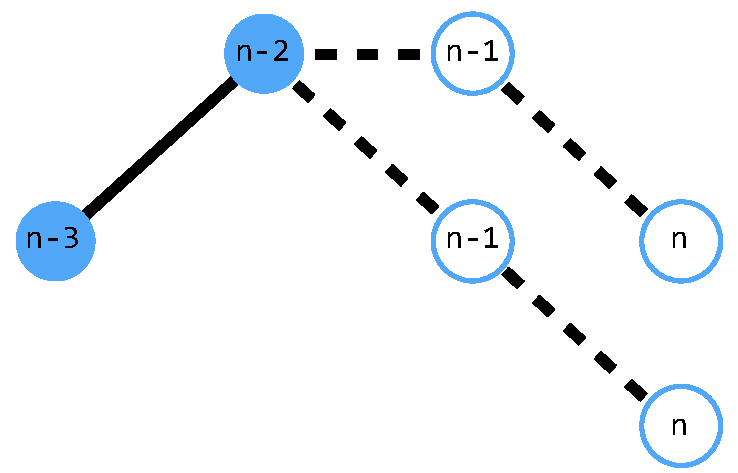
\includegraphics[width = 0.5\textwidth]{1Design/fig/peakReference.pdf}
        \caption{Peak blueprint. Straight lines symbolize a necessary relationship between data points. Dashed lines symbolize sufficient relationships between data points.}
        \label{fig:peakDetection}
\end{figure}

As seen on figure \ref{fig:peakDetection} we accept two different cases. Peaks with either one data point, or two data points at the top (a plateau). The subsequent data point must have a lower value. With this peak blueprint, the function \texttt{searchback} is only called twice during the test data: \texttt{ECG.txt}.

\subsubsection*{II. Update values: Not Rpeak}
If the peak satisfies the blueprint, but is weaker than \texttt{THRESHOLD1} (main threshold for peak amplitudes; used to discard peaks caused by noise), the peak is not saved as an Rpeak, but \texttt{THRESHOLD1} is updated accordingly. 

\subsubsection*{III. Calculate RR}
Once an accepted peak is stronger than \texttt{THRESHOLD1}, the interval between the current peak and previous Rpeak is calculated, also known as the the RR interval. This calculation uses a variable named \texttt{lastPeak} which keeps track of the iterations since last Rpeak. 

If the RR interval is between \texttt{RR\_LOW} and \texttt{RR\_HIGH} (variables to keep track of pulse rhythm) the function \texttt{updatePeak1} is called to save valid data. If the RR interval is not between these variables, the function \texttt{searchback} is called to investigate whether an Rpeak has been overlooked.

\subsubsection*{IV. Update values: peak1}
This function saves the peak as an Rpeak and adjusts variables tracking amplitude and rhythm to determine whether the patient has a stable heartbeat. This variable adjustment gives the program enough flexibility to handle the variations in the heartbeat caused by e.g. exercise and sleep.

\subsubsection*{V. Search backwards}
The \texttt{searchback} function is called if an irregularity in rhythm has occurred, and the RR interval is larger than the \texttt{RR\_MISS} variable. This suggests that an Rpeak is missed, forcing the program to look through previous peaks checking if a peak is stronger than \texttt{THRESHOLD2} (half the magnitude of \texttt{THRESHOLD1}), and if so, saving the peak as \texttt{peak2}.\\

The RR interval and \texttt{lastPeak} are adjusted according to the time between the last Rpeak and \texttt{peak2}.

\subsubsection*{VI. Update values: peak2}
Once a peak is found and stored as \texttt{peak2}, \texttt{updatePeak2} saves \texttt{peak2} as an Rpeak. This function is similar to \texttt{updatePeak1}, but instead of adjusting \texttt{RR\_LOW}, \texttt{RR\_HIGH} and \texttt{RR\_MISS} with respect to \texttt{RecentRR\_OK}, \texttt{updatePeak2} adjusts with respect to \texttt{RecentRR}. This way data from \texttt{searchback} is taken into account. See figure \ref{fig:QRS_flowchart}.
